In this example of acrobatic sports biomechanics, the goal was to maximize the twist rotation ($\phi$) of an 8-DoF model in a backward somersault. 
It illustrates \bioptim 's ability to handle quaternionic representations of rotations.
The model was composed of a 6-DoF root segment and two 1-DoF torque actuated shoulder joints.
Two different numerical descriptions of the root segment rotations were used: Euler angles and quaternions.
The objective function was as follows:

\begin{eqnarray}\label{eq:ocp_Trampo}
\mathcal{J} =  \int_0^T\underbrace{\omega_1 \dot{\phi}}_{\mathtt{MIN\_TWIST}}  + \underbrace{~\omega_2  \|\boldsymbol{\tau}\|^2}_{\mathtt{MIN\_ TORQUE}}~dt,
\end{eqnarray} 
with $\omega_1 = -1$ (resulting in the maximization of the first term) and $\omega_2 = 10^{-6}$, T is the duration of the movement and $\boldsymbol{\tau}$ is the torque control vector.
The first term of the objective function (Eq.~\ref{eq:ocp_Trampo}) corresponds to maximizing the change in twist rotation and the second term is for control regularization.
\begin{figure}[t!]
\centering
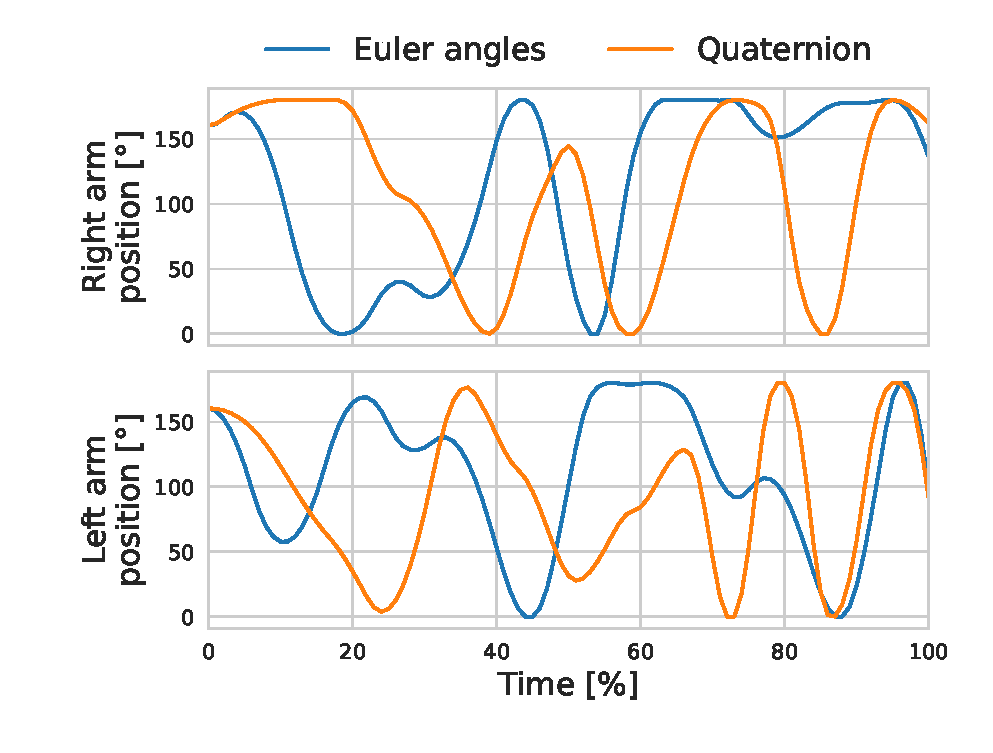
\includegraphics[width=\columnwidth]{figures/Twisting_armTech.eps}
\caption{Right (top) and left(bottom) arm kinematics of the twisting avatar for the euler angles (blues line) and the quaternion (orange line) representation of the orientation of the free base.}
\label{fig:Twist_armTech_graphs}
\vspace*{-1cm}
\end{figure}

The movement lasted for approximately 1 second and was discretized with 100 shooting nodes, a kinogram is presented in Fig.~\ref{fig:snapshots_quaternion_base_twisting_somersault}.
The optimal kinematics were different for the two types of models (Fig.~\ref{fig:Twist_armTech_graphs}) because of the presence of local minima.
However, both models take profits of a common biomechanical strategy (i.e. tilting the body to bring closer together the twist axis and the angular momentum vector) highlighting the equivalence of the two rotation representations.
Euler angles have the advantage to be easily interpretable, but they suffer from the loss of a DoF at the Gimbal lock (leading to numerical instabilities).
The use of a quaternion-based representation tackles this numerical stability issue when a joint is free to rotate on a three-dimensional range of motion.
Quaternion's integration must be handled with care~\cite{bailly2020optimal}.
Indeed, when representing orientations, quaternions must be unitary and thus belong to a constrained manifold (namely, the unit 3-sphere $S^3$). 
However, classical numerical integration schemes such as Runge–Kutta methods treat unit quaternions as if they were arbitrarily defined in $\mathbb{R}^4$.
To overcome this challenge, \bioptim performs a normalization after each Runge–Kutta iteration to project non-unitary quaternions onto $S^3$.

\begin{figure}[t!]
\centering
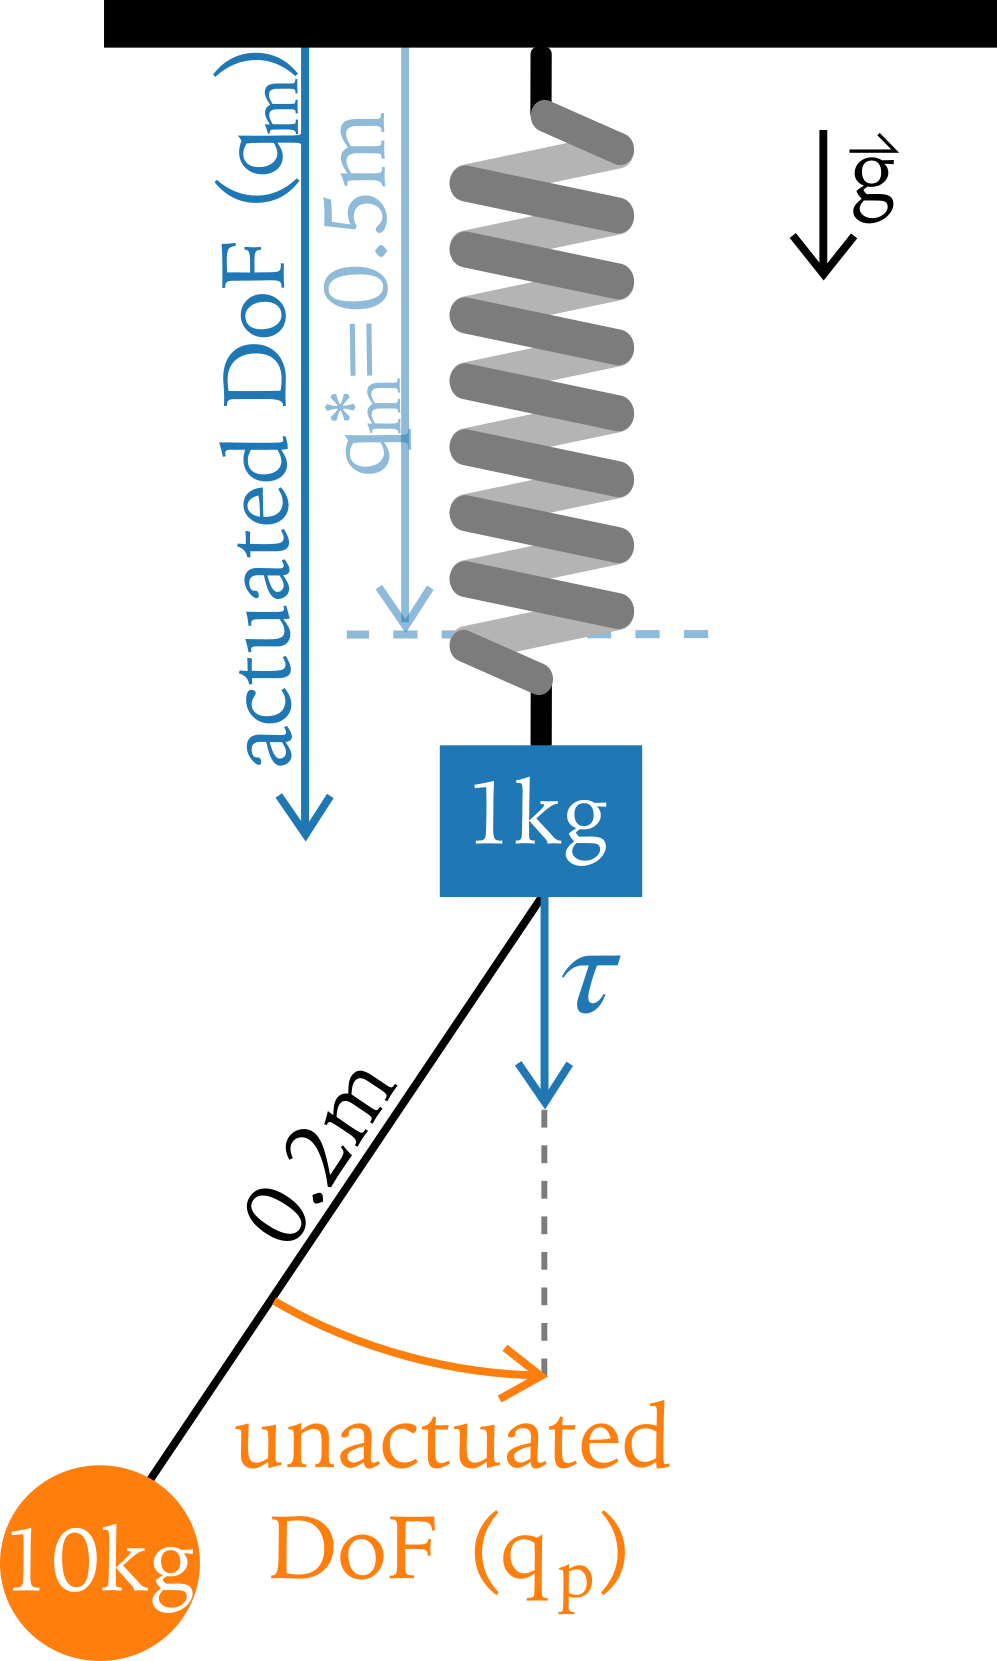
\includegraphics[width=0.35\columnwidth]{figures/Mass_Pendulum_Model_2.png}
\caption{Spring-mass-pendulum model of Ex.~\ref{ex:spring}.}
\label{fig:Mass_Pendulum_Model}
\end{figure}

\begin{figure}[h!]
\centering
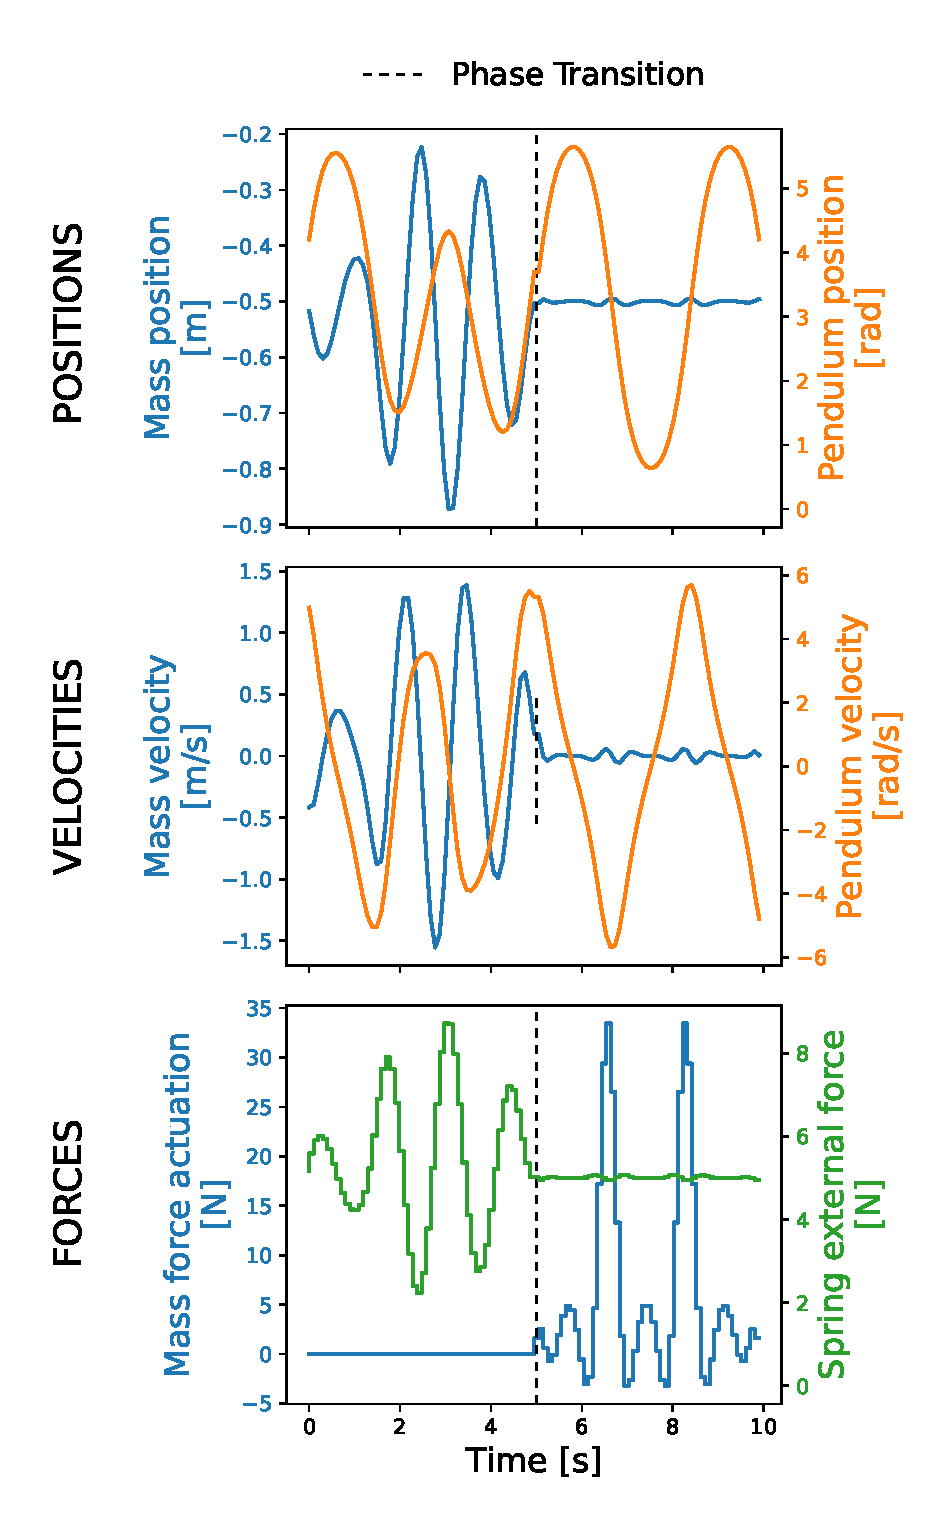
\includegraphics[width=\columnwidth]{figures/Mass_Pendulum_Fext.eps}
\caption{Two-phases kinematics of the mass-pendulum-spring system. Gray dashed lines show the phase transition, blue lines are related to the mass (position velocity and external force acting on it), red lines are related to the pendulum (position and velocity) and the green line depicts the spring force.}
\label{fig:Mass_Pendulum_Fext_graphs}
\vspace*{-0.5cm}
\end{figure}
